% !TEX program = xelatex
% 本文件为第四章独立解答。建议用 XeLaTeX 编译两次。
\documentclass[UTF8,a4paper,11pt]{ctexart}
\usepackage[a4paper,margin=2.15cm,headheight=16pt]{geometry}
\usepackage{amsmath,amssymb,mathtools,bm}
\usepackage{booktabs,longtable,array,enumitem}
\usepackage[most]{tcolorbox}
\usepackage{xcolor,fancyhdr,hyperref}
\usepackage{microtype}
\usepackage{tikz}
\definecolor{navy}{HTML}{264B86}
\definecolor{blue}{HTML}{356BA8}
\definecolor{pink}{HTML}{B84F82}
\definecolor{palepink}{HTML}{FBEAF2}
\definecolor{pale}{HTML}{EAF3FB}
\definecolor{gray}{HTML}{536171}
\hypersetup{colorlinks=true,linkcolor=navy,urlcolor=blue,pdftitle={常微分方程（第三版）第四章习题详细解答}}
\setlength{\parindent}{2em}
\setlength{\parskip}{0.28em}
\setlist[enumerate]{leftmargin=2.2em,itemsep=0.45em,topsep=0.35em}
\pagestyle{fancy}
\fancyhf{}
\fancyhead[L]{\small\color{gray}《常微分方程》（第三版）习题解答}
\fancyhead[R]{\small\color{pink}第四章·$n$ 阶线性微分方程}
\fancyfoot[C]{\small\thepage}
\renewcommand{\headrulewidth}{0.4pt}
\newcommand{\dd}{\,\mathrm d}
\newcommand{\e}{\mathrm e}
\newcommand{\R}{\mathbb R}
\newcommand{\note}[1]{\par\smallskip\noindent\textcolor{pink}{\bfseries 说明：}#1\par\smallskip}
\tcbset{
  exercisebox/.style={enhanced,breakable,arc=0pt,outer arc=0pt,
    boxsep=0pt,left=10pt,right=10pt,top=10pt,bottom=10pt,
    before skip=10pt,after skip=6pt,
    coltitle=navy,fonttitle=\bfseries,toptitle=6pt,bottomtitle=6pt,
    titlerule=0.4pt}
}
\newtcolorbox{problem}[1]{exercisebox,
  colback=white,colframe=blue,colbacktitle=pale,
  boxrule=0.55pt,leftrule=2pt,
  title={题目\quad #1}}
\newtcolorbox{solution}{exercisebox,
  colback=palepink!15!white,colframe=pink,colbacktitle=palepink,
  boxrule=0.45pt,leftrule=2pt,
  title={解答}}
\newtcolorbox{analysis}{exercisebox,
  colback=pale!30!white,colframe=blue,colbacktitle=pale,
  boxrule=0.4pt,leftrule=2pt,
  title={分析}}
\newcommand{\sect}[1]{\section*{\textcolor{navy}{习题 #1}}}

\begin{document}
\begin{center}
  {\LARGE\bfseries\color{navy}常微分方程（第三版）第四章习题解答\par}
  \vspace{0.35em}
  {\color{pink}$n$ 阶线性微分方程 · 习题 4.1--4.6\par}
\end{center}
\begin{center}
  \small\color{gray}本答案使用 AI 工具制作，请读者确认正确性后再使用。除非题目另有说明，本稿接受隐式解。
\end{center}

\sect{4.1}
\begin{problem}{4.1-1}
试讨论下列各函数组在它们的定义区间上是线性相关的还是线性无关的：
  \begin{enumerate}[label=(\arabic*)]
    \item $\sin 2t,\cos t,\sin t$；
    \item $x,\tan x$；
    \item $x^2-x+3,\,2x^2+x,\,2x+4$；
    \item $e^t,\,te^t,\,t^2e^t$。
  \end{enumerate}
\end{problem}

\begin{solution}
函数组的线性相关性使用常数系数，等式须在整个区间内成立。
\begin{enumerate}[label=(\arabic*)]
\item 计算朗斯基行列式：
\[
W(t)=\begin{vmatrix}
\sin2t&\cos t&\sin t\\
2\cos2t&-\sin t&\cos t\\
-4\sin2t&-\cos t&-\sin t
\end{vmatrix}=-3\sin2t.
\]
最后一步可将第一行加到第三行，再沿第三行展开。
在任一非退化区间内，都有 $\sin2t\ne0$ 的点，故 $W$ 在某点不为零，三个函数\textbf{线性无关}。

\item $\tan x$ 的各个定义区间为
$(-\pi/2+k\pi,\pi/2+k\pi)$，$k\in\mathbb Z$。
若 $ax+b\tan x\equiv0$，求两次导数得
\[
2b\sec^2x\tan x\equiv0.
\]
$\tan x$ 不会在一个区间内恒为零，而 $\sec^2x>0$，所以 $b=0$。
再由 $ax\equiv0$ 得 $a=0$，故两函数在各定义区间上\textbf{线性无关}。

\item 假设三个函数的一次常系数线性组合恒为零，比较 $x^2,x,1$ 的系数，得到
\[
\begin{pmatrix}1&2&0\\-1&1&2\\3&0&4\end{pmatrix}
\begin{pmatrix}c_1\\c_2\\c_3\end{pmatrix}=0.
\]
系数矩阵的行列式为 $24\ne0$，因此 $c_1=c_2=c_3=0$，三个函数\textbf{线性无关}。

\item 若 $c_1\e^t+c_2t\e^t+c_3t^2\e^t\equiv0$，除以处处非零的 $\e^t$ 得
$c_1+c_2t+c_3t^2\equiv0$。多项式在区间内恒为零，其系数全为零，故三个函数\textbf{线性无关}。
\end{enumerate}
\note{一般函数组的朗斯基行列式在某点为零，不能据此判定线性相关。（1）中 $W(0)=0$，但函数组仍线性无关。}
\end{solution}

\begin{problem}{4.1-2}
设在方程
  \[
    y''+p(x)y'+q(x)y=0
  \]
  中，$p(x)$ 在某区间 $I$ 上连续且恒不为零，试证它的任意两个线性无关的解的朗斯基行列式是区间 $I$ 上的严格单调函数。
\end{problem}

\begin{solution}
设两个线性无关解为 $y_1,y_2$，记
\[
W=y_1y_2'-y_1'y_2.
\]
用方程消去二阶导数，有
\[
W'=y_1y_2''-y_1''y_2=-p(x)W.
\]
由刘维尔公式，固定 $x_0\in I$ 后
\[
W(x)=W(x_0)\exp\left(-\int_{x_0}^xp(s)\dd s\right).
\]
基本解组的 $W(x_0)\ne0$，所以 $W$ 在 $I$ 上恒不为零且符号不变。
又 $p$ 连续并恒不为零，由介值定理，它在区间 $I$ 上也保持同一符号。
因而 $W'=-pW$ 恒为正或恒为负，故 $\boxed{W\text{ 在 }I\text{ 上严格单调}}$。
\end{solution}

\begin{problem}{4.1-3}
试证明：二阶线性齐次方程的任意两个线性无关解组的朗斯基行列式之比是一个不为零的常数。
\end{problem}

\begin{solution}
设两个基本解组的朗斯基行列式分别为 $W_1,W_2$。在同一点 $x_0$ 使用刘维尔公式，得
\[
W_j(x)=W_j(x_0)\exp\left(-\int_{x_0}^xp(s)\dd s\right),\qquad j=1,2.
\]
两者都处处非零，相除即得
\[
\boxed{\frac{W_1(x)}{W_2(x)}=\frac{W_1(x_0)}{W_2(x_0)}\ne0,}
\]
右侧与 $x$ 无关。
\end{solution}

\begin{problem}{4.1-4}
已知方程
  \[
    (x-1)y''-xy'+y=0
  \]
  的一个解 $y_1=x$，试求其通解。
\end{problem}

\begin{solution}
在 $x\ne1$ 的区间内，标准形式的 $y'$ 系数为 $p(x)=-x/(x-1)$。
由刘维尔公式，与已知解 $y_1=x$ 配对的朗斯基行列式可写成
\[
W=xy'-y=K(x-1)\e^x,
\]
因为 $\int x/(x-1)\dd x=x+\ln|x-1|$，各区间上的符号可以并入常数 $K$。
在 $x\ne0$ 处令 $y=xz$，便有 $W=x^2z'$，故
\[
z'=K\frac{(x-1)\e^x}{x^2}
=K\left(\frac{\e^x}{x}\right)'.
\]
积分得 $z=C_1+K\e^x/x$，从而
\[
\boxed{y=C_1x+C_2\e^x.}
\]
两解的朗斯基行列式为 $(x-1)\e^x$，在 $x\ne1$ 的区间上不为零，故上述式子包含全部解。
\note{推导中的 $x=0$ 只是除以已知解时产生的临时限制，最后的公式可直接延伸到 $x=0$。
$x=1$ 是原方程最高阶系数的零点，通解定理先应用于它的两侧；所得函数在该点仍满足未除以 $x-1$ 的原方程。}
\end{solution}

\begin{problem}{4.1-5}
已知方程
  \[
    (1-\ln x)y''+\frac{1}{x}y'-\frac{1}{x^2}y=0
  \]
  的一个解 $y_1=\ln x$，试求其通解。
\end{problem}

\begin{solution}
实数范围先要求 $x>0$。在 $x\ne\e$ 的区间上，将方程化为标准形式，其 $y'$ 系数为
\[
p(x)=\frac{1}{x(1-\ln x)},\qquad
\int p(x)\dd x=-\ln|1-\ln x|.
\]
因此刘维尔公式给出
\[
W=(\ln x)y'-\frac{y}{x}=K(\ln x-1).
\]
在 $\ln x\ne0$ 处令 $y=(\ln x)z$，则
\[
W=(\ln x)^2z',\qquad
z'=K\frac{\ln x-1}{(\ln x)^2}
=K\left(\frac{x}{\ln x}\right)'.
\]
积分并还原 $y$，得到
\[
\boxed{y=C_1\ln x+C_2x.}
\]
两解的朗斯基行列式为 $\ln x-1$，故这是 $(0,\e)$ 或 $(\e,+\infty)$ 上的通解。
推导中排除的 $x=1$ 可由最后的公式延伸补回；公式在 $x=\e$ 处也满足原来的退化方程。
\end{solution}

\begin{problem}{4.1-6}
在方程
  \[
    y''+p(x)y'+q(x)y=0
  \]
  中，当系数满足什么条件时，其基本解组构成的朗斯基行列式等于常数？
\end{problem}

\begin{solution}
基本解组的朗斯基行列式 $W$ 处处非零，且满足 $W'=-p(x)W$。
因此
\[
W\text{ 为常数}\ \Longleftrightarrow\ W'\equiv0
\ \Longleftrightarrow\ p(x)\equiv0.
\]
所以所求条件为 $\boxed{p\equiv0}$；$q$ 除通常的连续性要求外，无须附加条件。
这里的常数 $W$ 必为非零常数。
\end{solution}

\begin{problem}{4.1-7}
设 $y_1(x)$ 是 $n$ 阶线性齐次方程
  \[
    y^{(n)}+a_1(x)y^{(n-1)}+\cdots+a_{n-1}(x)y'+a_n(x)y=0
  \]
  的一个非零解。试证明：利用线性变换 $y=y_1(x)z$ 可将已知方程化为 $n-1$ 阶的齐次方程。
\end{problem}

\begin{solution}
取一个 $y_1(x)\ne0$ 的区间，令 $y=y_1z$。
记 $a_0=1$，由莱布尼茨公式，
\[
\begin{aligned}
L[y_1z]
&=\sum_{j=0}^na_j(x)(y_1z)^{(n-j)}\\
&=\sum_{j=0}^na_j(x)\sum_{k=0}^{n-j}
\binom{n-j}{k}y_1^{(n-j-k)}z^{(k)}.
\end{aligned}
\]
其中所有不含 $z$ 的导数的项之和为 $zL[y_1]=0$。
把其余项按 $z^{(k)}$ 合并，得到
\[
y_1z^{(n)}+b_{n-1}(x)z^{(n-1)}+\cdots+b_1(x)z'=0,
\]
这里
\[
b_k(x)=\sum_{j=0}^{n-k}a_j(x)\binom{n-j}{k}y_1^{(n-j-k)},
\qquad 1\le k\le n-1.
\]
方程中没有 $z$ 本身。再令 $u=z'$，便得到
\[
\boxed{y_1u^{(n-1)}+b_{n-1}u^{(n-2)}+\cdots+b_1u=0,}
\]
除以 $y_1$ 后就是 $n-1$ 阶线性齐次方程。
求出 $u$ 后，积分 $z=\int u\dd x+C$，再乘回 $y_1$ 即可还原 $y$。
\note{“非零解”指不恒为零，并不排除它有零点。变换作为可逆的降阶步骤，须在 $y_1\ne0$ 的区间上使用；不能在其零点处直接除以 $y_1$。}
\end{solution}

\begin{problem}{4.1-8}
已知方程
  \[
    x^3y'''-3x^2y''+6xy'-6y=0
  \]
  的两个特解 $y_1=x,y_2=x^2$，求其通解。
\end{problem}

\begin{solution}
在 $x\ne0$ 的区间上用已知解 $x$ 降阶，令 $y=xz$。有
\[
y'=z+xz',\quad y''=2z'+xz'',\quad y'''=3z''+xz'''.
\]
代入后各项相消：
\[
\begin{aligned}
&x^3(3z''+xz''')-3x^2(2z'+xz'')
+6x(z+xz')-6xz\\
&\hspace{3em}=x^4z'''=0.
\end{aligned}
\]
因此 $z'''=0$，逐次积分得 $z=C_1+C_2x+C_3x^2$，故
\[
\boxed{y=C_1x+C_2x^2+C_3x^3.}
\]
三解的朗斯基行列式为
\[
\begin{vmatrix}x&x^2&x^3\\1&2x&3x^2\\0&2&6x\end{vmatrix}=2x^3,
\]
在 $x\ne0$ 时非零，所以没有遗漏解；所得多项式也可以延伸到 $x=0$。
\end{solution}

\begin{problem}{4.1-9}
设
  \[
  \Delta(x)=
  \begin{vmatrix}
  a_{11}(x)&a_{12}(x)&a_{13}(x)\\
  a_{21}(x)&a_{22}(x)&a_{23}(x)\\
  a_{31}(x)&a_{32}(x)&a_{33}(x)
  \end{vmatrix},
  \]
  求证：
  \[
  \frac{d\Delta(x)}{dx}
  =
  \begin{vmatrix}
  a'_{11}(x)&a'_{12}(x)&a'_{13}(x)\\
  a_{21}(x)&a_{22}(x)&a_{23}(x)\\
  a_{31}(x)&a_{32}(x)&a_{33}(x)
  \end{vmatrix}
  +
  \begin{vmatrix}
  a_{11}(x)&a_{12}(x)&a_{13}(x)\\
  a'_{21}(x)&a'_{22}(x)&a'_{23}(x)\\
  a_{31}(x)&a_{32}(x)&a_{33}(x)
  \end{vmatrix}
  +
  \begin{vmatrix}
  a_{11}(x)&a_{12}(x)&a_{13}(x)\\
  a_{21}(x)&a_{22}(x)&a_{23}(x)\\
  a'_{31}(x)&a'_{32}(x)&a'_{33}(x)
  \end{vmatrix}.
  \]
  并试证对 $n$ 阶行列式也有类似结果。
\end{problem}

\begin{solution}
设所有矩阵元素可微。行列式的排列展开式为
\[
\Delta(x)=\sum_{\sigma\in S_n}\operatorname{sgn}(\sigma)
\prod_{i=1}^na_{i,\sigma(i)}(x).
\]
这里 $S_n$ 是 $1,\ldots,n$ 的所有排列的集合。
这是有限项之和，逐项求导并使用乘积求导法则，得
\[
\Delta'
=\sum_{r=1}^n\sum_{\sigma\in S_n}\operatorname{sgn}(\sigma)
a'_{r,\sigma(r)}\prod_{i\ne r}a_{i,\sigma(i)}.
\]
对每个固定的 $r$，内层和恰是将原矩阵的第 $r$ 行求导、其余各行保持原状后的行列式。因此
\[
\boxed{\Delta'=\sum_{r=1}^n
\det\bigl(A\text{ 的第 }r\text{ 行替换为其导数所得的矩阵}\bigr).}
\]
取 $n=3$ 就得到题中三项相加的公式，这也同时证明了 $n$ 阶的推广。
\end{solution}

\begin{problem}{4.1-10}
设 $p(x),q(x),f(x)$ 在 $[0,1]$ 上连续，试证明，方程
  \[
    y''+p(x)y'+q(x)y=f(x)
  \]
  满足条件 $y(0)=y(1)=0$ 的解唯一的充要条件是：方程
  \[
    y''+p(x)y'+q(x)y=0
  \]
  只有零解满足条件 $y(0)=y(1)=0$。
\end{problem}

\begin{solution}
记 $L[y]=y''+py'+qy$。

\textbf{必要性。} 若非齐次边值问题有唯一解 $y_p$，而齐次方程有满足两端零条件的非零解 $z$，则 $y_p+z$ 也是同一非齐次边值问题的解，与唯一性矛盾。因此这种 $z$ 不存在。

\textbf{充分性。} 下面同时证明解的存在性和唯一性。
由初值问题定理，存在 $u,v$ 满足
\[
\begin{cases}L[u]=f,\\u(0)=u'(0)=0,\end{cases}
\qquad
\begin{cases}L[v]=0,\\v(0)=0,\ v'(0)=1.\end{cases}
\]
$v$ 是非零解。若 $v(1)=0$，它便是题设排除的齐次边值非零解，故 $v(1)\ne0$。
所有满足 $L[y]=f$、$y(0)=0$ 的解都可写成
\[
y=u+cv.
\]
事实上，对于给定的 $y$，取 $c=y'(0)$，$y-u-cv$ 满足齐次方程及零初值，因而恒为零。
条件 $y(1)=0$ 唯一地确定
\[
c=-\frac{u(1)}{v(1)}.
\]
故所求边值解存在且唯一，具体为
\[
\boxed{y(x)=u(x)-\frac{u(1)}{v(1)}v(x).}
\]
\end{solution}

\begin{problem}{4.1-11}
用常数变易法求方程
  \[
    y''-y=\frac{2e^x}{e^x-1}
  \]
  的通解。
\end{problem}

\begin{solution}
直接代入可验证 $y_1=\e^x,y_2=\e^{-x}$ 是齐次方程的解，它们的朗斯基行列式为 $-2$。
令非齐次特解为 $y_p=u(x)\e^x+v(x)\e^{-x}$，常数变易法给出
\[
\begin{cases}
u'\e^x+v'\e^{-x}=0,\\
u'\e^x-v'\e^{-x}=\dfrac{2\e^x}{\e^x-1}.
\end{cases}
\]
解得
\[
u'=\frac1{\e^x-1},\qquad v'=-\frac{\e^{2x}}{\e^x-1}.
\]
积分时令 $r=\e^x$，有
\[
\begin{aligned}
u&=\int\frac{\dd r}{r(r-1)}=\ln|\e^x-1|-x,\\
v&=-\int\frac{r}{r-1}\dd r=-\e^x-\ln|\e^x-1|.
\end{aligned}
\]
其中积分常数并入齐次解。于是通解为
\[
\boxed{y=C_1\e^x+C_2\e^{-x}
+(\e^x-\e^{-x})\ln|\e^x-1|-x\e^x-1.}
\]
原方程在 $x=0$ 无定义，应分别在 $x<0$ 或 $x>0$ 的区间上取解。
\end{solution}

\begin{problem}{4.1-12}
在方程
  \[
    y''+3y'+2y=f(x)
  \]
  中，$f(x)$ 在 $[a,+\infty)$ 上连续，且
  \[
    \lim_{x\to+\infty}f(x)=0,
  \]
  试证明，对于方程的任一解 $y(x)$，均有
  \[
    \lim_{x\to+\infty}y(x)=0.
  \]
\end{problem}

\begin{solution}
直接验证可知 $\e^{-x},\e^{-2x}$ 是对应齐次方程的基本解组。
令 $y=u\e^{-x}+v\e^{-2x}$，常数变易法给出
\[
u'\e^{-x}+v'\e^{-2x}=0,\qquad
-u'\e^{-x}-2v'\e^{-2x}=f(x).
\]
所以 $u'=\e^xf(x)$、$v'=-\e^{2x}f(x)$。从 $a$ 积分后，通解写成
\[
\begin{aligned}
y(x)={}&C_1\e^{-(x-a)}+C_2\e^{-2(x-a)}\\
&+\int_a^x\bigl[\e^{-(x-s)}-\e^{-2(x-s)}\bigr]f(s)\dd s.
\end{aligned}
\]
记 $K(r)=\e^{-r}-\e^{-2r}$（$r\ge0$），则
\[
K(r)\ge0,\qquad \int_0^{\infty}K(r)\dd r=\frac12.
\]
给定 $\varepsilon>0$，选 $R\ge a$ 使 $s\ge R$ 时 $|f(s)|<\varepsilon$。
对于 $x\ge R$，将积分分成 $[a,R]$ 和 $[R,x]$ 两段。
令 $M=\max_{[a,R]}|f|$，第一段满足
\[
\left|\int_a^RK(x-s)f(s)\dd s\right|
\le M\int_a^R\e^{-(x-s)}\dd s
=M(\e^{R-x}-\e^{a-x})\longrightarrow0.
\]
第二段满足
\[
\left|\int_R^xK(x-s)f(s)\dd s\right|
\le\varepsilon\int_0^{x-R}K(r)\dd r\le\frac\varepsilon2.
\]
因为 $\varepsilon$ 任意，非齐次积分项趋于零；两个齐次项也趋于零。因此
\[
\boxed{\lim_{x\to+\infty}y(x)=0.}
\]
\end{solution}

\sect{4.2}
\begin{problem}{4.2-1}
试求下列各方程的通解：
  \begin{enumerate}[label=(\arabic*)]
    \item $y''+y'+20y=0$；
    \item $y'''-y=0$；
    \item $y^{(4)}+y=0$；
    \item $y''-2y'+y=0$；
    \item $y^{(4)}-y''=0$；
    \item $y'''-y''-y'+y=0$；
    \item $y^{(6)}-2y^{(4)}-y''+2y=0$。
  \end{enumerate}
\end{problem}

\begin{solution}
将 $y=\e^{\lambda x}$ 代入得到特征方程。实根 $\lambda$ 为 $m$ 重根时，对应
$\e^{\lambda x},x\e^{\lambda x},\ldots,x^{m-1}\e^{\lambda x}$；
共轭根 $\alpha\pm\mathrm i\beta$ 对应实解 $\e^{\alpha x}\cos\beta x$、$\e^{\alpha x}\sin\beta x$。
\begin{enumerate}[label=(\arabic*)]
\item 特征方程为 $\lambda^2+\lambda+20=0$，根为
\[
\lambda=-\frac12\pm\frac{\sqrt{79}}2\mathrm i.
\]
因此
\[
\boxed{y=\e^{-x/2}\left(C_1\cos\frac{\sqrt{79}x}{2}
+C_2\sin\frac{\sqrt{79}x}{2}\right).}
\]
\note{教材第 137 页原题是 $y''+y'+20y=0$，整理版误多写了一个导数符号。
参考书给出的 $C_1\e^{-4x}+C_2\e^{-5x}$ 也不满足教材此题，故这里按原方程重新计算。}

\item 特征多项式
\[
\lambda^3-1=(\lambda-1)(\lambda^2+\lambda+1)
\]
的根为 $1,-1/2\pm\sqrt3\mathrm i/2$，所以
\[
\boxed{y=C_1\e^x+\e^{-x/2}
\left(C_2\cos\frac{\sqrt3x}{2}+C_3\sin\frac{\sqrt3x}{2}\right).}
\]

\item 由
\[
\lambda^4+1=(\lambda^2-\sqrt2\lambda+1)(\lambda^2+\sqrt2\lambda+1),
\]
得四个根 $\pm1/\sqrt2\pm\mathrm i/\sqrt2$。故
\[
\boxed{\begin{aligned}
y={}&\e^{x/\sqrt2}\left(C_1\cos\frac{x}{\sqrt2}+C_2\sin\frac{x}{\sqrt2}\right)\\
&+\e^{-x/\sqrt2}\left(C_3\cos\frac{x}{\sqrt2}+C_4\sin\frac{x}{\sqrt2}\right).
\end{aligned}}
\]

\item 特征多项式为 $(\lambda-1)^2$，$1$ 为二重根，故
\[
\boxed{y=(C_1+C_2x)\e^x.}
\]

\item $\lambda^4-\lambda^2=\lambda^2(\lambda-1)(\lambda+1)$。
零根为二重根，其余根为 $1,-1$，故
\[
\boxed{y=C_1+C_2x+C_3\e^x+C_4\e^{-x}.}
\]

\item
\[
\lambda^3-\lambda^2-\lambda+1
=(\lambda-1)(\lambda^2-1)=(\lambda-1)^2(\lambda+1).
\]
所以
\[
\boxed{y=(C_1+C_2x)\e^x+C_3\e^{-x}.}
\]

\item 特征多项式分解为
\[
\begin{aligned}
\lambda^6-2\lambda^4-\lambda^2+2
&=(\lambda^2-2)(\lambda^4-1)\\
&=(\lambda^2-2)(\lambda-1)(\lambda+1)(\lambda^2+1).
\end{aligned}
\]
六个单根为 $\sqrt2,-\sqrt2,1,-1,\mathrm i,-\mathrm i$，因而
\[
\boxed{y=C_1\e^{\sqrt2x}+C_2\e^{-\sqrt2x}
+C_3\e^x+C_4\e^{-x}+C_5\cos x+C_6\sin x.}
\]
\note{教材第 138 页原题是六阶方程，整理版中的 $(16),(14)$ 应分别为 $(6),(4)$；新题干已经恢复。}
\end{enumerate}
\end{solution}

\begin{problem}{4.2-2}
试求下面方程满足给定初值条件的解：
  \begin{enumerate}[label=(\arabic*)]
    \item
    \[
      y''-3y'+2y=0;\qquad y(0)=2,\quad y'(0)=-3;
    \]
    \item
    \[
      y''+y'=0;\qquad y(0)=2,\quad y'(0)=5;
    \]
    \item
    \[
      y''+4y'+4y=0,\qquad y(2)=4,\quad y'(2)=0.
    \]
  \end{enumerate}
\end{problem}

\begin{solution}
\begin{enumerate}[label=(\arabic*)]
\item 特征方程为 $(\lambda-1)(\lambda-2)=0$，故
$y=C_1\e^x+C_2\e^{2x}$。初值给出
\[
C_1+C_2=2,\qquad C_1+2C_2=-3,
\]
解得 $C_1=7,C_2=-5$，所以 $\boxed{y=7\e^x-5\e^{2x}}$。

\item 特征方程为 $\lambda(\lambda+1)=0$，故 $y=C_1+C_2\e^{-x}$。
由 $C_1+C_2=2$、$-C_2=5$，得
\[
\boxed{y=7-5\e^{-x}.}
\]

\item 特征根为二重根 $-2$。为方便代入初值，令 $h=x-2$，写成
\[
y=(A+Bh)\e^{-2h}.
\]
有 $y(2)=A$、$y'(2)=B-2A$，所以 $A=4,B=8$，从而
\[
\boxed{y=\bigl(4+8(x-2)\bigr)\e^{-2(x-2)}.}
\]
\end{enumerate}
\end{solution}

\begin{problem}{4.2-3}
求分别满足下列条件的方程的通解，并确定相应的方程：
  \begin{enumerate}[label=(\arabic*)]
    \item 已知某一三阶常系数线性齐次方程有特解 $5xe^x,e^{2x}$；
    \item 已知某一三阶常系数线性齐次方程有特解 $e^{-2x},\sin 3x$；
    \item 已知某一四阶常系数线性齐次方程的特征方程只有特征根 $0,\pm i$。
  \end{enumerate}
\end{problem}

\begin{solution}
按本章约定，考虑实常系数、最高阶系数化为 $1$ 的方程，记其特征多项式为 $P(\lambda)$。
\begin{enumerate}[label=(\arabic*)]
\item $5x\e^x$ 是解，等价于 $x\e^x$ 是解。利用
\[
P(D)[x\e^x]=\e^x\bigl[xP(1)+P'(1)\bigr],\qquad D=\frac{\dd}{\dd x},
\]
可知 $P(1)=P'(1)=0$，即 $1$ 至少是二重根。
又 $\e^{2x}$ 是解，故 $P(2)=0$。方程只有三阶，于是
\[
P(\lambda)=(\lambda-1)^2(\lambda-2)
=\lambda^3-4\lambda^2+5\lambda-2.
\]
所以方程和通解分别为
\[
\boxed{y'''-4y''+5y'-2y=0,\qquad
y=(C_1+C_2x)\e^x+C_3\e^{2x}.}
\]

\item $\e^{-2x}$ 是解，故 $-2$ 为特征根。
$\sin3x$ 是解，实系数条件下 $3\mathrm i,-3\mathrm i$ 都是特征根。
三个根已经用满三阶，所以
\[
P(\lambda)=(\lambda+2)(\lambda^2+9)
=\lambda^3+2\lambda^2+9\lambda+18.
\]
得到
\[
\boxed{\begin{gathered}
y'''+2y''+9y'+18y=0,\\
y=C_1\e^{-2x}+C_2\cos3x+C_3\sin3x.
\end{gathered}}
\]

\item 因系数为实数，$\mathrm i,-\mathrm i$ 的重数相等。
若它们的共同重数为 $m\ge1$、零根重数为 $r\ge1$，则 $r+2m=4$，只能有 $m=1,r=2$。
因此
\[
P(\lambda)=\lambda^2(\lambda^2+1),
\]
所求为
\[
\boxed{y^{(4)}+y''=0,\qquad
y=C_1+C_2x+C_3\cos x+C_4\sin x.}
\]
\end{enumerate}
\end{solution}

\begin{problem}{4.2-4}
设 $y(x)$ 在 $(-\infty,+\infty)$ 内具有连续的二阶导数，满足
  \[
    3y(x)=1-\int_0^x\bigl[y''(t)+y'(t)+4y(t)\bigr]\,dt,
  \]
  且 $y'(0)=0$，求 $y(x)$。
\end{problem}

\begin{solution}
先令 $x=0$，得 $y(0)=1/3$。由于被积函数连续，对原等式求导：
\[
3y'=-y''-y'-4y,
\]
即
\[
y''+4y'+4y=0,\qquad y(0)=\frac13,\quad y'(0)=0.
\]
特征根为二重根 $-2$，故 $y=(C_1+C_2x)\e^{-2x}$。
初值给出 $C_1=1/3$、$C_2-2C_1=0$，于是
\[
\boxed{y(x)=\frac13(1+2x)\e^{-2x}.}
\]
为确认求导没有丢失原等式，记
\[
H(x)=3y(x)+\int_0^x[y''(t)+y'(t)+4y(t)]\dd t.
\]
由所得微分方程 $H'=0$，且 $H(0)=1$，故 $H\equiv1$，原积分等式成立。
\end{solution}

\begin{problem}{4.2-5}
考虑方程
  \[
    y''+py'+qy=0,
  \]
  \begin{enumerate}[label=(\arabic*)]
    \item 若 $p=0$，$q$ 为何值时，该方程存在满足 $y'(0)=y(1)=0$ 的非零解？
    \item $p,q$ 取何值时，当 $x\to+\infty$ 时，该方程的一切解都趋于零？
    \item $p,q$ 取何值时，该方程的一切解在 $[a,+\infty)$ 上有界，其中 $a$ 是某确定的常数？
    \item $p,q$ 取何值时，该方程的一切解都是 $x$ 的周期函数？
  \end{enumerate}
\end{problem}

\begin{solution}
以下 $p,q$ 均为实常数。特征方程为
\[
\lambda^2+p\lambda+q=0,\qquad
\lambda_{1,2}=\frac{-p\pm\sqrt{p^2-4q}}2.
\]
\begin{enumerate}[label=(\arabic*)]
\item 此处 $p=0$。若 $q>0$，记 $\mu=\sqrt q$，通解为
$y=A\cos\mu x+B\sin\mu x$。由 $y'(0)=0$ 得 $B=0$，再由 $y(1)=0$ 得
$A\cos\mu=0$。要有非零解，须且只须 $\cos\mu=0$，即
\[
\boxed{q=\left(n+\frac12\right)^2\pi^2,\qquad n=0,1,2,\ldots.}
\]
相应非零解为 $y=A\cos[(n+1/2)\pi x]$，$A\ne0$。
若 $q=0$，通解为 $A+Bx$，两条件使 $A=B=0$；若 $q<0$，令 $\mu=\sqrt{-q}$，由 $y'(0)=0$ 得 $y=A\cosh\mu x$，再因 $\cosh\mu>0$ 得 $A=0$。
\note{参考书给出的 $q=n^2\pi^2$ 对应不同的边界条件；按本题的 $y'(0)=y(1)=0$，应得到上面的半整数频率。}

\item 全部解趋于零，等价于两个特征根的实部都为负。
实根情况下还要考虑重根所带的 $x$ 因子，但 $x\e^{\lambda x}\to0$ 对 $\lambda<0$ 仍成立。
若 $p>0,q>0$，当根为实数时，由和为 $-p<0$、积为 $q>0$ 可知两个根均负；当根非实时，实部均为 $-p/2<0$。
反过来，两个根实部均负时，根的和与积分别给出 $p>0,q>0$。
故所求条件为
\[
\boxed{p>0,\qquad q>0.}
\]

\item 两个根实部均负时，所有解有界。如果有零实部的根，它必须是单根，才能避免 $x$ 因子引起增长。
在 $p>0,q>0$ 之外，还有两种允许情形：
\[
\begin{array}{c|c|c}
\text{条件}&\text{特征根}&\text{通解形式}\\ \hline
p>0,\ q=0&0,-p&A+B\e^{-px}\\
p=0,\ q>0&\pm\mathrm i\sqrt q&A\cos\sqrt qx+B\sin\sqrt qx
\end{array}
\]
两类解在 $[a,+\infty)$ 上都有界。
若 $q<0$，必有正实根；若 $p<0$，两根实部之和为 $-p>0$，必有正实部的根；这两种情况都有无界解。
余下的 $p=q=0$ 有解 $y=x$，同样不符合要求。
因此充要条件为
\[
\boxed{p>0,\ q\ge0\quad\text{或}\quad p=0,\ q>0.}
\]

\item 若 $p=0,q>0$，所有解都是正弦、余弦的线性组合，公共周期可取 $2\pi/\sqrt q$，所以满足要求。
反过来，非零实部的特征根会产生非周期的指数解；零根若与非零实根配对，也有非周期解；二重零根产生 $y=x$。
故全部解为周期函数，只能对应一对非零纯虚根 $\pm\mathrm i\beta$。
由两根的和、积得
\[
\boxed{p=0,\qquad q>0.}
\]
\end{enumerate}
\end{solution}

\sect{4.3}
\begin{problem}{4.3-1}
求下列方程的通解：
  \begin{enumerate}[label=(\arabic*)]
    \item $y''-7y'+12y=5$；
    \item $y''+4y=8$；
    \item $y''+y'+y=3e^{2x}$；
    \item $y''-6y'+9y=4e^{3x}$；
    \item $y''-8y'+7y=3x^2+7x+8$；
    \item $y''-2y'+4y=(x+2)e^{3x}$；
    \item $y''+6y'+13y=(x^2-5x+2)e^x$；
    \item $y''+y=5\sin 2x$；
    \item $y''-2y'+10y=x\cos 2x$；
    \item $y''+9y=18\cos 3x-30\sin 3x$。
  \end{enumerate}
\end{problem}

\begin{solution}
各题通解均为齐次通解 $y_h$ 加一个非齐次特解 $y_p$。
计算指数型特解时可用乘积求导公式：若 $y_p=\e^{\alpha x}v$，则
\[
y_p''+ay_p'+by_p
=\e^{\alpha x}\bigl[v''+(2\alpha+a)v'+(\alpha^2+a\alpha+b)v\bigr].
\]
\begin{enumerate}[label=(\arabic*)]
\item 齐次特征方程 $(\lambda-3)(\lambda-4)=0$，故
$y_h=C_1\e^{3x}+C_2\e^{4x}$。
设常数特解 $y_p=A$，代入得 $12A=5$。因此
\[
\boxed{y=C_1\e^{3x}+C_2\e^{4x}+\frac5{12}.}
\]

\item 齐次根为 $\pm2\mathrm i$，$y_h=C_1\cos2x+C_2\sin2x$。
设 $y_p=A$，由 $4A=8$ 得 $A=2$，所以
\[
\boxed{y=C_1\cos2x+C_2\sin2x+2.}
\]

\item 齐次根为 $-1/2\pm\sqrt3\mathrm i/2$。
右端指数 $2$ 不是特征根，设 $y_p=A\e^{2x}$，代入得 $(4+2+1)A=3$，即 $A=3/7$。
故
\[
\boxed{y=\e^{-x/2}\left(C_1\cos\frac{\sqrt3x}{2}+C_2\sin\frac{\sqrt3x}{2}\right)+\frac37\e^{2x}.}
\]

\item 齐次根 $3$ 为二重根，$y_h=(C_1+C_2x)\e^{3x}$。
右端也含 $\e^{3x}$，特解须取 $y_p=Ax^2\e^{3x}$。
令 $v=Ax^2$ 后左边变成 $\e^{3x}v''=2A\e^{3x}$，故 $A=2$。于是
\[
\boxed{y=(C_1+C_2x)\e^{3x}+2x^2\e^{3x}.}
\]

\item 齐次根为 $1,7$。设 $y_p=Ax^2+Bx+D$，代入并比较系数：
\[
7A=3,\qquad 7B-16A=7,\qquad 2A-8B+7D=8.
\]
依次得 $A=3/7,B=97/49,D=1126/343$，故
\[
\boxed{y=C_1\e^x+C_2\e^{7x}+\frac37x^2+\frac{97}{49}x+\frac{1126}{343}.}
\]

\item 齐次根为 $1\pm\sqrt3\mathrm i$。
设 $y_p=\e^{3x}(Ax+B)$，令 $v=Ax+B$，待定系数满足
\[
v''+4v'+7v=x+2,\qquad 7A=1,\quad4A+7B=2.
\]
所以 $A=1/7,B=10/49$，得到
\[
\boxed{y=\e^x(C_1\cos\sqrt3x+C_2\sin\sqrt3x)
+\e^{3x}\left(\frac{x}{7}+\frac{10}{49}\right).}
\]

\item 齐次特征方程为 $(\lambda+3)^2+4=0$，故
$y_h=\e^{-3x}(C_1\cos2x+C_2\sin2x)$。
设 $y_p=\e^xv$，$v=Ax^2+Bx+D$，则
\[
v''+8v'+20v=x^2-5x+2.
\]
比较系数得
\[
20A=1,\qquad16A+20B=-5,\qquad2A+8B+20D=2,
\]
从而 $A=1/20,B=-29/100,D=211/1000$。因此
\[
\boxed{\begin{aligned}
y={}&\e^{-3x}(C_1\cos2x+C_2\sin2x)\\
&+\e^x\left(\frac{x^2}{20}-\frac{29x}{100}+\frac{211}{1000}\right).
\end{aligned}}
\]
\note{参考书给出的非齐次多项式系数有误；这里的系数由上面三个代数等式确定。}

\item 齐次根为 $\pm\mathrm i$。由于 $\pm2\mathrm i$ 不是特征根，设 $y_p=A\sin2x$，得 $(-4+1)A=5$。所以
\[
\boxed{y=C_1\cos x+C_2\sin x-\frac53\sin2x.}
\]

\item 齐次特征方程为 $(\lambda-1)^2+9=0$，故
$y_h=\e^x(C_1\cos3x+C_2\sin3x)$。
右端频率 $2$ 不对应特征根，设
\[
y_p=(Ax+B)\cos2x+(Cx+D)\sin2x.
\]
分别比较余弦、正弦中 $x$ 项与常数项，得到
\[
\begin{cases}
6A-4C=1,\\4A+6C=0,\\
-2A+6B+4C-4D=0,\\
-4A+4B-2C+6D=0.
\end{cases}
\]
前两式给出 $A=3/26,C=-1/13$；代回后两式，得 $B=29/338,D=-1/169$。
故
\[
\boxed{\begin{aligned}
y={}&\e^x(C_1\cos3x+C_2\sin3x)\\
&+\left(\frac{3x}{26}+\frac{29}{338}\right)\cos2x
-\left(\frac{x}{13}+\frac1{169}\right)\sin2x.
\end{aligned}}
\]
\note{参考书在齐次部分误写了频率 $2$；由特征根 $1\pm3\mathrm i$，齐次部分的频率应为 $3$。}

\item 齐次根为 $\pm3\mathrm i$，与右端频率相同，故设
\[
y_p=x(A\cos3x+B\sin3x).
\]
计算得 $y_p''+9y_p=-6A\sin3x+6B\cos3x$。
比较系数，得 $A=5,B=3$，于是
\[
\boxed{y=C_1\cos3x+C_2\sin3x+x(5\cos3x+3\sin3x).}
\]
\end{enumerate}
\end{solution}

\begin{problem}{4.3-2}
设 $f(x)$ 是定义在 $(-\infty,+\infty)$ 内的连续函数且满足
  \[
    f(x)=e^x-\int_0^x(x-t)f(t)\,dt,
  \]
  求 $f(x)$。
\end{problem}

\begin{solution}
令 $G(x)=\int_0^x(x-t)f(t)\dd t$，也可写成
\[
G(x)=x\int_0^xf(t)\dd t-\int_0^xtf(t)\dd t.
\]
因为 $f$ 连续，求导得 $G'=\int_0^xf(t)\dd t$、$G''=f(x)$。
由 $f=\e^x-G$ 可知 $f$ 实际上二阶连续可导，且满足
\[
f''+f=\e^x,\qquad f(0)=1,\quad f'(0)=1.
\]
设特解 $A\e^x$，得到 $A=1/2$，所以
\[
f=C_1\cos x+C_2\sin x+\frac12\e^x.
\]
初值给出 $C_1=C_2=1/2$，故
\[
\boxed{f(x)=\frac12(\cos x+\sin x+\e^x).}
\]
反过来，对此函数定义 $H=f-\e^x+G$，由方程得 $H''=0$，初值得 $H(0)=H'(0)=0$，所以 $H\equiv0$，原积分方程也成立。
\end{solution}

\begin{problem}{4.3-3}
设 $f(x)$ 二阶连续可导，$f(0)=0,f'(0)=1$，且
  \[
    [xy(x+y)-f(x)y]\,dx+[f'(x)+x^2y]\,dy=0
  \]
  是全微分方程，求 $f(x)$ 及此全微分方程的通解。
\end{problem}

\begin{solution}
记
\[
M=x^2y+xy^2-f(x)y,\qquad N=f'(x)+x^2y.
\]
全微分条件 $M_y=N_x$ 给出
\[
x^2+2xy-f(x)=f''(x)+2xy,
\]
即 $f''+f=x^2$。设多项式特解为 $Ax^2+Bx+D$，得 $A=1,B=0,D=-2$，所以
\[
f=A_1\cos x+A_2\sin x+x^2-2.
\]
由 $f(0)=0,f'(0)=1$ 得 $A_1=2,A_2=1$，于是
\[
\boxed{f(x)=2\cos x+\sin x+x^2-2.}
\]
再求原全微分方程的势函数 $U$。先从 $U_y=N$ 积分：
\[
U=f'(x)y+\frac12x^2y^2+h(x).
\]
其 $x$ 导数为 $f''(x)y+xy^2+h'$；由 $f''=x^2-f$ 与 $U_x=M$ 得 $h'=0$。
常数并入右端后，原方程的通解为
\[
\boxed{\frac12x^2y^2+(2x-2\sin x+\cos x)y=C.}
\]
\end{solution}

\begin{problem}{4.3-4}
设 $f(x)$ 二阶连续可导，且使得曲线积分
  \[
    \int_{\gamma}\bigl[f'(x)+6f(x)+e^{-2x}\bigr]y\,dx+f'(x)\,dy
  \]
  与路径无关，求 $f(x)$。
\end{problem}

\begin{solution}
曲线积分与路径无关，其被积微分形式应满足全微分条件。
令
\[
M=[f'(x)+6f(x)+\e^{-2x}]y,\qquad N=f'(x),
\]
由 $M_y=N_x$ 得
\[
f''-f'-6f=\e^{-2x}.
\]
齐次特征多项式 $(\lambda-3)(\lambda+2)$，所以
$f_h=C_1\e^{-2x}+C_2\e^{3x}$。
由于 $-2$ 是单根，取特解 $f_p=Ax\e^{-2x}$，代入得
$-5A\e^{-2x}=\e^{-2x}$，即 $A=-1/5$。
因此
\[
\boxed{f(x)=C_1\e^{-2x}+C_2\e^{3x}-\frac{x}{5}\e^{-2x}.}
\]
对这些函数，$f''=f'+6f+\e^{-2x}$，原微分形式恰为
$\dd(f'(x)y)$，故所得条件也足以保证积分与路径无关。
\end{solution}

\begin{problem}{4.3-5}
考虑方程
  \[
    y''+8y'+7y=q(x),
  \]
  其中 $q(x)$ 在 $[0,+\infty)$ 上连续。
  \begin{enumerate}[label=(\arabic*)]
    \item 若 $q(x)$ 在 $[0,+\infty)$ 上有界，则该方程的任一解在 $[0,+\infty)$ 上有界；
    \item 若 $\displaystyle\lim_{x\to+\infty}q(x)=0$，则该方程任一解 $y(x)$ 满足
    \[
      \lim_{x\to+\infty}y(x)=0.
    \]
  \end{enumerate}
\end{problem}

\begin{solution}
齐次根为 $-1,-7$。由常数变易法，任意解均可写成
\[
y(x)=C_1\e^{-x}+C_2\e^{-7x}
+\int_0^xK(x-s)q(s)\dd s,
\qquad K(r)=\frac{\e^{-r}-\e^{-7r}}6.
\]
这里 $r\ge0$ 时 $K(r)\ge0$，并且 $\int_0^{\infty}K(r)\dd r=1/7$。
\begin{enumerate}[label=(\arabic*)]
\item 若 $|q(s)|\le M$，则
\[
\left|\int_0^xK(x-s)q(s)\dd s\right|
\le M\int_0^xK(r)\dd r\le\frac M7.
\]
齐次部分在 $x\ge0$ 上也有界，所以
$|y(x)|\le |C_1|+|C_2|+M/7$，结论成立。

\item 给定 $\varepsilon>0$，选 $R\ge0$ 使 $s\ge R$ 时 $|q(s)|<\varepsilon$。
令 $M_R=\max_{[0,R]}|q|$。对 $x\ge R$，有
\[
\begin{aligned}
\left|\int_0^RK(x-s)q(s)\dd s\right|
&\le\frac{M_R}{6}\int_0^R\e^{-(x-s)}\dd s\longrightarrow0,\\
\left|\int_R^xK(x-s)q(s)\dd s\right|
&\le\varepsilon\int_0^{x-R}K(r)\dd r\le\frac\varepsilon7.
\end{aligned}
\]
由 $\varepsilon$ 任意，积分项趋于零，齐次部分也趋于零。故
\[
\boxed{\lim_{x\to+\infty}y(x)=0.}
\]
\end{enumerate}
\end{solution}

\sect{4.4}
\begin{problem}{4.4-1}
一质量为 $p=4\,\mathrm{kg}$ 的物体挂在弹簧下端，它使弹簧的长度增长 $1\,\mathrm{cm}$，假定弹簧的上端有一转动机产生铅直调和振动
  \[
    y=2\sin 30t\ \mathrm{cm},
  \]
  并在初始时刻 $t=0$ 时，重物处于静止状态，试求该重物的运动规律。
\end{problem}

\begin{solution}
取向下为正，$x(t)$ 表示重物相对于原静平衡位置的位移，以米计；弹簧上端位移为
$b(t)=0.02\sin30t$ 米。记弹性系数为 $K$，静伸长量为 $\delta=0.01$ 米。
由静平衡 $K\delta=mg$，得 $K/m=g/\delta$。支点移动后，弹簧伸长量为 $\delta+x-b$，故牛顿第二定律给出
\[
mx''=mg-K(\delta+x-b)=-Kx+Kb.
\]
令 $\omega_0=\sqrt{g/\delta}$，则
\[
x''+\omega_0^2x=0.02\omega_0^2\sin30t.
\]
按参考书约定，初始静止取为 $x(0)=x'(0)=0$。
当 $\omega_0\ne30$ 时，设特解 $A\sin30t$，得
\[
A=\frac{0.02\omega_0^2}{\omega_0^2-900}.
\]
齐次解为 $B\cos\omega_0t+D\sin\omega_0t$。两初值依次给出 $B=0$、$D=-30A/\omega_0$，因此运动规律为
\[
\boxed{x(t)=\frac{0.02\omega_0^2}{\omega_0^2-900}
\left(\sin30t-\frac{30}{\omega_0}\sin\omega_0t\right)\ \mathrm m.}
\]
若取 $g=9.8\,\mathrm{m/s^2}$，则 $\omega_0=\sqrt{980}\,\mathrm{s^{-1}}$，也可用厘米写成
\[
\boxed{x(t)=24.5\left(\sin30t-\frac{30}{\sqrt{980}}\sin(\sqrt{980}\,t)\right)\ \mathrm{cm}.}
\]
若恰有 $\omega_0=30$，取共振特解 $-0.01\omega_0t\cos\omega_0t$，再配合初值得
\[
x(t)=0.01\bigl(\sin30t-30t\cos30t\bigr)\ \mathrm m.
\]
\note{“静止”若仅指初速度为零，题目还缺初始位置。这里按初始静平衡解释；若初始位移为 $x_0$，只需在上述结果上加 $x_0\cos\omega_0t$。
建模时已将题中的厘米统一换成米，质量 $4\,\mathrm{kg}$ 在 $K/m=g/\delta$ 中消去了。}
\end{solution}

\begin{problem}{4.4-2}
一质量为 $m$ 的质点由静止开始沉入液体中，当下沉时，液体的反作用与下沉的速度成正比，求此质点的运动规律。
\end{problem}

\begin{solution}
取向下为正，沉入点为位移原点。令液体反作用为 $-\kappa x'$，其中 $\kappa>0$。
根据牛顿第二定律，
\[
mx''=mg-\kappa x',\qquad x(0)=0,\quad x'(0)=0.
\]
令 $v=x'$，先解一阶线性方程
\[
v'+\frac\kappa m v=g.
\]
乘以积分因子 $\e^{\kappa t/m}$，由 $v(0)=0$ 得
\[
v(t)=\frac{mg}{\kappa}\left(1-\e^{-\kappa t/m}\right).
\]
再从 $0$ 到 $t$ 积分，得到运动规律
\[
\boxed{x(t)=\frac{mg}{\kappa}t
-\frac{m^2g}{\kappa^2}\left(1-\e^{-\kappa t/m}\right),\qquad t\ge0.}
\]
速度由零逐渐趋于 $mg/\kappa$，这是阻力与重力平衡时的速度。
\end{solution}

\begin{problem}{4.4-3}
在 $LC$ 电路中（如图 4--7 所示），先将开关拨到“1”处，对电容器进行充电到电源电压 $U_0$，然后再将开关拨到“2”处，如果
  \[
    C=2\times10^{-9}\,\mathrm{F},\qquad L=5\times10^{-4}\,\mathrm{H},
  \]
  求此 $LC$ 电路中的电流 $i(t)$ 和电容器两端的电压 $u_C(t)$。
\begin{center}
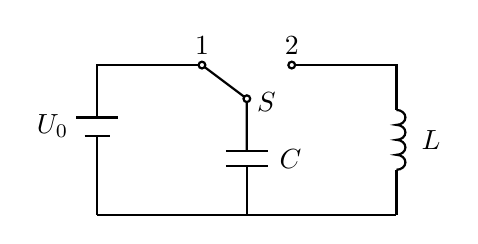
\begin{tikzpicture}[scale=0.95,line width=0.8pt]
\draw (0,0)--(4,0);
\draw (0,0)--(0,1.05);
\draw (-0.17,1.05)--(0.17,1.05);
\draw (-0.28,1.3)--(0.28,1.3);
\draw (0,1.3)--(0,2)--(1.4,2);
\draw (2,0)--(2,0.65);
\draw (1.72,0.65)--(2.28,0.65);
\draw (1.72,0.85)--(2.28,0.85);
\draw (2,0.85)--(2,1.55)--(1.4,2);
\draw (4,0)--(4,0.6);
\draw (4,0.6)
  arc[start angle=-90,end angle=90,x radius=0.12,y radius=0.1]
  arc[start angle=-90,end angle=90,x radius=0.12,y radius=0.1]
  arc[start angle=-90,end angle=90,x radius=0.12,y radius=0.1]
  arc[start angle=-90,end angle=90,x radius=0.12,y radius=0.1];
\draw (4,1.4)--(4,2)--(2.6,2);
\foreach \x in {1.4,2.6} {\draw[fill=white] (\x,2) circle(0.045);}
\draw[fill=white] (2,1.55) circle(0.045);
\node[above] at (1.4,2) {$1$}; \node[above] at (2.6,2) {$2$};
\node[right] at (2,1.5) {$S$}; \node[left] at (-0.25,1.18) {$U_0$};
\node[right] at (2.3,0.75) {$C$}; \node[right] at (4.2,1) {$L$};
\end{tikzpicture}
\par\small 图 4--7\quad 充电与 $LC$ 振荡电路示意
\end{center}
\end{problem}

\begin{solution}
令 $q(t)$ 为初始带正电的电容极板上的电荷，取 $u_C=q/C$。
以电流由该极板流出、经电感返回另一极板的方向为正，则 $i=-q'$。
充电结束时 $q(0)=CU_0$，电感中的初始电流为 $0$，故 $q'(0)=0$。
开关拨到 $2$ 后，电容与电感组成闭合回路。由
$u_C=L i'$ 得
\[
Lq''+\frac qC=0,\qquad q(0)=CU_0,\quad q'(0)=0.
\]
记 $\omega=1/\sqrt{LC}$，解得
\[
q=CU_0\cos\omega t,\qquad
u_C=U_0\cos\omega t,\qquad
i=CU_0\omega\sin\omega t.
\]
代入数值得 $LC=10^{-12}$、$\omega=10^6\,\mathrm{s^{-1}}$，且 $C\omega=2\times10^{-3}$，因此
\[
\boxed{u_C(t)=U_0\cos(10^6t),\qquad
i(t)=\frac{U_0}{500}\sin(10^6t).}
\]
当 $U_0$ 用伏特表示、$t$ 用秒表示时，电压单位为伏特，电流单位为安培。
\note{电流的正负号依赖方向约定。若定义 $i=q'$，电流公式前须加负号；参考书把 $i=q'$ 与上面的正号同时写出，符号约定不一致。}
\end{solution}

\begin{problem}{4.4-4}
设 $\varphi(t)$ 是
  \[
    x''+k^2x=f(t)
  \]
  的解，其中 $k$ 为常数，$f(t)$ 在 $[0,+\infty)$ 上连续。证明：
  \begin{enumerate}[label=(\arabic*)]
    \item 当 $k\ne0$ 时，能够选择常数 $c_1,c_2$ 的值，使得
    \[
      \varphi(t)
      =c_1\cos kt+\frac{c_2}{k}\sin kt
      +\frac{1}{k}\int_0^t\sin[k(t-s)]f(s)\,ds,
      \qquad t\in[0,+\infty);
    \]
    \item 当 $k=0$ 时，该方程的通解可表为
    \[
      \varphi(t)=c_1+c_2t+\int_0^t(t-s)f(s)\,ds,
      \qquad t\in[0,+\infty),
    \]
    其中 $c_1,c_2$ 为任意常数。
  \end{enumerate}
\end{problem}

\begin{solution}
\begin{enumerate}[label=(\arabic*)]
\item 当 $k\ne0$ 时，齐次基本解组可取 $\cos kt,\sin kt/k$，其朗斯基行列式为 $1$。
设 $\varphi=a(t)\cos kt+b(t)\sin kt/k$，常数变易法给出
\[
\begin{cases}
a'\cos kt+b'\sin kt/k=0,\\
-ka'\sin kt+b'\cos kt=f(t).
\end{cases}
\]
解得 $a'=-f(t)\sin kt/k$、$b'=f(t)\cos kt$。
从 $0$ 积分，并记 $c_1=a(0),c_2=b(0)$，于是
\[
\begin{aligned}
\varphi(t)={}&c_1\cos kt+\frac{c_2}{k}\sin kt\\
&+\frac1k\int_0^t
\bigl[\sin kt\cos ks-\cos kt\sin ks\bigr]f(s)\dd s.
\end{aligned}
\]
使用正弦差角公式便得到题中的表示：
\[
\boxed{\varphi(t)=c_1\cos kt+\frac{c_2}{k}\sin kt
+\frac1k\int_0^t\sin[k(t-s)]f(s)\dd s.}
\]
这里 $c_1=\varphi(0),c_2=\varphi'(0)$。

\item 当 $k=0$ 时，方程为 $\varphi''=f(t)$。先积分一次：
\[
\varphi'(t)=c_2+\int_0^tf(s)\dd s.
\]
再积分一次得
\[
\boxed{\varphi(t)=c_1+c_2t+\int_0^t(t-s)f(s)\dd s.}
\]
最后一项的导数为 $\int_0^tf(s)\dd s$，故该式确实包含所有两次积分所得的解。
两个常数分别是初始位移、初始速度，均可任取。
\end{enumerate}
\end{solution}

\sect{4.5}
\begin{problem}{4.5-1}
用拉普拉斯变换求解下列初值问题：
  \begin{enumerate}[label=(\arabic*)]
    \item
    \[
      \dot{x}-x=e^{2t},\qquad x(0)=0;
    \]
    \item
    \[
      \ddot{x}+2\dot{x}+x=e^{-t},\qquad x(0)=\dot{x}(0)=0;
    \]
    \item
    \[
      \dddot{x}+3\ddot{x}+3\dot{x}+x=1,\qquad
      x(0)=\dot{x}(0)=\ddot{x}(0)=0;
    \]
    \item
    \[
      \ddot{x}+a^2x=b\sin at,\qquad x(0)=x_0,\quad \dot{x}(0)=\dot{x}_0;
    \]
    \item
    \[
      y''-3y'+2y=e^{3t},\qquad y(0)=1,\quad y'(0)=0;
    \]
    \item
    \[
      y''-2y'+y=te^t,\qquad y(0)=0,\quad y'(0)=0.
    \]
  \end{enumerate}
\end{problem}

\begin{solution}
记 $X(s)=\mathcal L\{x(t)\}$，$Y(s)=\mathcal L\{y(t)\}$。
使用导数的变换公式
\[
\begin{aligned}
\mathcal L\{x'\}&=sX-x(0),\\
\mathcal L\{x''\}&=s^2X-sx(0)-x'(0),\\
\mathcal L\{x'''\}&=s^3X-s^2x(0)-sx'(0)-x''(0),
\end{aligned}
\]
以及 $\mathcal L\{t^n\e^{at}\}=n!/(s-a)^{n+1}$。
\begin{enumerate}[label=(\arabic*)]
\item 变换后 $(s-1)X=1/(s-2)$，所以
\[
X=\frac1{(s-1)(s-2)}=\frac1{s-2}-\frac1{s-1}.
\]
取逆变换，得 $\boxed{x(t)=\e^{2t}-\e^t}$。

\item 因两初值均为零，变换后
\[
(s+1)^2X=\frac1{s+1},\qquad X=\frac1{(s+1)^3}.
\]
故 $\boxed{x(t)=\tfrac12t^2\e^{-t}}$。

\item 三个初值均为零，变换后 $(s+1)^3X=1/s$，故
\[
X=\frac1{s(s+1)^3}
=\frac1s-\frac1{s+1}-\frac1{(s+1)^2}-\frac1{(s+1)^3}.
\]
逐项取逆变换，得
\[
\boxed{x(t)=1-\left(1+t+\frac{t^2}{2}\right)\e^{-t}.}
\]

\item 先设 $a\ne0$，记 $v_0=\dot x_0$。变换后
\[
(s^2+a^2)X-sx_0-v_0=\frac{ba}{s^2+a^2},
\]
所以
\[
X=x_0\frac{s}{s^2+a^2}+v_0\frac1{s^2+a^2}
+\frac{ba}{(s^2+a^2)^2}.
\]
最后一项可用
\[
\mathcal L\{t\cos at\}=\frac{s^2-a^2}{(s^2+a^2)^2}
\]
来求逆变换，因为
\[
\frac{a}{(s^2+a^2)^2}
=\frac1{2a^2}\left(\frac{a}{s^2+a^2}
-a\frac{s^2-a^2}{(s^2+a^2)^2}\right).
\]
故
\[
\boxed{x(t)=x_0\cos at+\frac{v_0}{a}\sin at
+\frac{b}{2a^2}\bigl(\sin at-at\cos at\bigr),\quad a\ne0.}
\]
若 $a=0$，原方程退化为 $x''=0$，变换为 $X=x_0/s+v_0/s^2$，从而 $\boxed{x=x_0+v_0t}$。

\item 代入初值，变换后
\[
(s^2-3s+2)Y-s+3=\frac1{s-3}.
\]
所以
\[
\begin{aligned}
Y&=\frac{s-3}{(s-1)(s-2)}
+\frac1{(s-1)(s-2)(s-3)}\\
&=\frac{5}{2(s-1)}-\frac2{s-2}+\frac1{2(s-3)}.
\end{aligned}
\]
取逆变换得到
\[
\boxed{y(t)=\frac52\e^t-2\e^{2t}+\frac12\e^{3t}.}
\]

\item 初值均为零，右端 $t\e^t$ 的变换为 $1/(s-1)^2$，因此
\[
(s-1)^2Y=\frac1{(s-1)^2},\qquad Y=\frac1{(s-1)^4}.
\]
故 $\boxed{y(t)=\tfrac16t^3\e^t}$。
\end{enumerate}
\end{solution}

\begin{problem}{4.5-2}
应用拉普拉斯变换求解下列方程组：
  \begin{enumerate}[label=(\arabic*)]
    \item
    \[
    \begin{cases}
      \dot{x}+y=-p\sin\omega t,\\
      x-\dot{y}=-p\cos\omega t,\\
      x(0)=1,\ y(0)=0;
    \end{cases}
    \]
    \item
    \[
    \begin{cases}
      \dot{x}+x+y=t^2,\\
      \dot{y}+y+z=2t,\\
      \dot{z}+z=t;
    \end{cases}
    \]
    \item
    \[
    \begin{cases}
      \ddot{x}+\ddot{y}+x+y=\sin t,\\
      \dot{x}+2\dot{y}=e^{-t};
    \end{cases}
    \]
    \item
    \[
    \begin{cases}
      \ddot{x}+6x+7y=0,\\
      \ddot{y}+3x+2y=2t.
    \end{cases}
    \]
  \end{enumerate}
\end{problem}

\begin{solution}
以下记 $X=\mathcal L\{x\}$、$Y=\mathcal L\{y\}$、$Z=\mathcal L\{z\}$。
未指定初值的方程组，通过任取初值求得通解。
\begin{enumerate}[label=(\arabic*)]
\item 代入给定初值，变换得到
\[
\begin{cases}
sX-1+Y=-\dfrac{p\omega}{s^2+\omega^2},\\[5pt]
X-sY=-\dfrac{ps}{s^2+\omega^2}.
\end{cases}
\]
解这个二元代数方程组：
\[
\begin{aligned}
X&=\frac{s}{s^2+1}
-\frac{p(1+\omega)s}{(s^2+1)(s^2+\omega^2)},\\
Y&=\frac1{s^2+1}
+\frac{p(s^2-\omega)}{(s^2+1)(s^2+\omega^2)}.
\end{aligned}
\]
当 $\omega\ne1$ 时，可改写为
\[
\begin{aligned}
X&=\frac{s}{s^2+1}+\frac{p}{1-\omega}
\left(\frac{s}{s^2+1}-\frac{s}{s^2+\omega^2}\right),\\
Y&=\frac1{s^2+1}+\frac{p}{1-\omega}
\left(\frac1{s^2+1}-\frac{\omega}{s^2+\omega^2}\right).
\end{aligned}
\]
逐项取逆变换得
\[
\boxed{\begin{aligned}
x(t)&=\cos t+\frac{p}{1-\omega}(\cos t-\cos\omega t),\\
y(t)&=\sin t+\frac{p}{1-\omega}(\sin t-\sin\omega t),\qquad \omega\ne1.
\end{aligned}}
\]
当 $\omega=1$ 时，应从未分解的像函数计算：
\[
X=\frac{s}{s^2+1}-\frac{2ps}{(s^2+1)^2},\qquad
Y=\frac1{s^2+1}+p\frac{s^2-1}{(s^2+1)^2}.
\]
由 $\mathcal L\{t\sin t\}=2s/(s^2+1)^2$、
$\mathcal L\{t\cos t\}=(s^2-1)/(s^2+1)^2$ 得
\[
\boxed{x(t)=\cos t-pt\sin t,\qquad
y(t)=\sin t+pt\cos t,\qquad\omega=1.}
\]

\item 设任意初值 $x(0)=\alpha,y(0)=\beta,z(0)=\gamma$。
由最后一式开始，变换后依次有
\[
\begin{aligned}
(s+1)Z&=\gamma+\frac1{s^2},\\
(s+1)Y&=\beta+\frac2{s^2}-Z,\\
(s+1)X&=\alpha+\frac2{s^3}-Y.
\end{aligned}
\]
记 $K=\gamma+1$，依次化简像函数：
\[
\begin{aligned}
Z&=\frac{K}{s+1}+\frac1{s^2}-\frac1s,\\
Y&=\frac1{s^2}+\frac{\beta}{s+1}-\frac{K}{(s+1)^2},\\
X&=\frac2{s^3}-\frac3{s^2}+\frac3s
+\frac{\alpha-3}{s+1}-\frac{\beta}{(s+1)^2}+\frac{K}{(s+1)^3}.
\end{aligned}
\]
取逆变换，并记 $C_1=K/2,C_2=-\beta,C_3=\alpha-3$，得
\[
\boxed{\begin{aligned}
x(t)&=\e^{-t}(C_1t^2+C_2t+C_3)+t^2-3t+3,\\
y(t)&=\e^{-t}(-2C_1t-C_2)+t,\\
z(t)&=2C_1\e^{-t}+t-1.
\end{aligned}}
\]
初值与三个 $C_j$ 之间的变换可逆，所以三个常数都可任取。
\note{教材第 159 页末式右端为 $t$，整理版误抄成了 $1$；这里的题干和解答均按 $t$ 恢复。}

\item 取 $x(0)=a,y(0)=b,y'(0)=c$。第二式在 $t=0$ 还要求 $x'(0)=1-2c$，故只有三个独立初值。
由第二式的变换，
\[
s(X+2Y)=a+2b+\frac1{s+1}.
\]
令 $K=a+2b+1$，则
\[
X+2Y=\frac K s-\frac1{s+1}.
\]
第一式变换为
\[
(s^2+1)(X+Y)=s(a+b)+1-c+\frac1{s^2+1}.
\]
用前一式消去 $X$，得到
\[
Y=\frac{sb+c}{s^2+1}
+\frac{K}{s(s^2+1)}
-\frac2{(s+1)(s^2+1)}-\frac1{(s^2+1)^2}.
\]
所需分解及逆变换为
\[
\begin{aligned}
\frac1{s(s^2+1)}&=\frac1s-\frac{s}{s^2+1},\\
-\frac2{(s+1)(s^2+1)}&=-\frac1{s+1}+\frac{s-1}{s^2+1},\\
\mathcal L^{-1}\left\{\frac1{(s^2+1)^2}\right\}
&=\frac12(\sin t-t\cos t).
\end{aligned}
\]
所以 $y=K+(b-K+1)\cos t+(c-3/2)\sin t-\e^{-t}+t\cos t/2$。
再由 $x+2y=K-\e^{-t}$ 求出 $x$，将任意常数重新记为 $C_1,C_2,C_3$，得到
\[
\boxed{\begin{aligned}
x(t)&=-C_1-2C_2\cos t-2C_3\sin t+\e^{-t}-t\cos t,\\
y(t)&=C_1+C_2\cos t+C_3\sin t-\e^{-t}+\frac t2\cos t.
\end{aligned}}
\]
这里 $C_1=K,C_2=b-K+1,C_3=c-3/2$，均可任取。
\note{本题首式已按确认更正为 $\ddot x+\ddot y+x+y=\sin t$；整理版原来把 $\ddot y$ 误写成了 $\dot y$。}

\item 先作可逆的线性变换
\[
u=\frac{3x-7y}{10},\qquad v=\frac{x+y}{10},\qquad
x=u+7v,\quad y=-u+3v.
\]
将原两式按这两个线性组合相加，得到
\[
u''-u=-\frac75t,\qquad v''+9v=\frac15t.
\]
取任意初值 $u(0)=a,u'(0)=b,v(0)=c,v'(0)=d$。
记 $U=\mathcal L\{u\},V=\mathcal L\{v\}$，变换得
\[
\begin{aligned}
U&=\frac{sa+b}{s^2-1}-\frac7{5s^2(s^2-1)}
=\frac{sa+b-7/5}{s^2-1}+\frac7{5s^2},\\
V&=\frac{sc+d}{s^2+9}+\frac1{5s^2(s^2+9)}
=\frac{sc+d-1/45}{s^2+9}+\frac1{45s^2}.
\end{aligned}
\]
分别取逆变换，将任意常数改记为 $C_j$，有
\[
u=C_1\e^t+C_2\e^{-t}+\frac75t,\qquad
v=C_3\cos3t+C_4\sin3t+\frac{t}{45}.
\]
还原变量得到通解
\[
\boxed{\begin{aligned}
x(t)&=C_1\e^t+C_2\e^{-t}+7C_3\cos3t+7C_4\sin3t+\frac{14}{9}t,\\
y(t)&=-C_1\e^t-C_2\e^{-t}+3C_3\cos3t+3C_4\sin3t-\frac43t.
\end{aligned}}
\]
\end{enumerate}
\end{solution}

\sect{4.6}
\begin{problem}{4.6-1}
试用幂级数解法求解方程
$y''+xy'+y=0$；
\end{problem}

\begin{solution}
在 $x=0$ 的邻域设普通幂级数
\[
y=\sum_{n=0}^{\infty}a_nx^n.
\]
代入方程并统一为 $x^n$ 的系数，得
\[
\sum_{n=0}^{\infty}
\bigl[(n+2)(n+1)a_{n+2}+(n+1)a_n\bigr]x^n=0.
\]
因此递推式为
\[
\boxed{a_{n+2}=-\frac{a_n}{n+2},\qquad n\ge0.}
\]
偶数、奇数系数分别由 $a_0,a_1$ 决定：
\[
a_{2k}=\frac{(-1)^ka_0}{2^kk!},\qquad
a_{2k+1}=\frac{(-1)^ka_1}{1\cdot3\cdot5\cdots(2k+1)}.
\]
于是通解为
\[
\boxed{y=C_1\e^{-x^2/2}
+C_2\sum_{k=0}^{\infty}\frac{(-1)^kx^{2k+1}}{1\cdot3\cdot5\cdots(2k+1)}.}
\]
这里第一项来自 $\sum(-1)^kx^{2k}/(2^kk!)$。
第二个级数相邻项绝对值之比为 $|x|^2/(2k+3)\to0$，故两级数对所有实数 $x$ 收敛，可以在有界区间上逐项求导。
两解在 $0$ 处的初值分别为 $(y,y')=(1,0),(0,1)$，所以线性无关，确实构成基本解组。
\note{原式也可写成 $(y'+xy)'=0$。用一阶线性方程的积分因子，可把同一通解写为
$y=\e^{-x^2/2}\bigl(C_1+C_2\int_0^x\e^{s^2/2}\dd s\bigr)$，这与上述级数一致。}
\end{solution}

\begin{problem}{4.6-2}
试用幂级数解法求解方程
$y''+x^2y'=0$；
\end{problem}

\begin{solution}
设 $y=\sum_{n=0}^{\infty}a_nx^n$。代入得
\[
\sum_{n=0}^{\infty}(n+2)(n+1)a_{n+2}x^n
+\sum_{n=2}^{\infty}(n-1)a_{n-1}x^n=0.
\]
最低两次幂给出 $a_2=a_3=0$；其余项给出
\[
a_{n+2}=-\frac{n-1}{(n+2)(n+1)}a_{n-1},\qquad n\ge2.
\]
所以除常数项外，只有下标为 $3k+1$ 的系数可能非零。递推可化简为
\[
\begin{aligned}
a_{3k+1}
&=a_1(-1)^k\prod_{j=0}^{k-1}
\frac{3j+1}{(3j+4)(3j+3)}\\
&=\frac{(-1)^ka_1}{3^kk!(3k+1)},\qquad k\ge0,
\end{aligned}
\]
其中 $k=0$ 时空积为 $1$。因此
\[
\boxed{y=C_1+C_2\sum_{k=0}^{\infty}
\frac{(-1)^kx^{3k+1}}{3^kk!(3k+1)}.}
\]
相邻非零项绝对值之比为
$|x|^3(3k+1)/[3(k+1)(3k+4)]\to0$，故级数对一切实数 $x$ 收敛。
两解在 $0$ 处的初值为 $(1,0),(0,1)$，故上述式子是通解。
\note{级数的导数为 $\e^{-x^3/3}$，所以也可写成
$y=C_1+C_2\int_0^x\e^{-s^3/3}\dd s$。}
\end{solution}

\begin{problem}{4.6-3}
试用幂级数解法求解方程
$2xy''+(1-2x)y'-y=0$；
\end{problem}

\begin{solution}
$x=0$ 是最高阶系数的零点，设广义幂级数，先在 $x>0$ 上计算：
\[
y=x^r\sum_{n=0}^{\infty}a_nx^n,\qquad a_0\ne0.
\]
代入 $2xy''+(1-2x)y'-y=0$。最低次幂 $x^{r-1}$ 的系数为
\[
r(2r-1)a_0=0,
\]
故指标根为 $r=0,1/2$。对 $n\ge1$，比较 $x^{n+r-1}$ 的系数：
\[
(n+r)(2n+2r-1)a_n-(2n+2r-1)a_{n-1}=0.
\]
对上述两个指标根，因子 $2n+2r-1\ne0$，所以
\[
a_n=\frac{a_{n-1}}{n+r}.
\]
当 $r=0$，取 $a_0=1$ 得 $a_n=1/n!$，第一解为 $y_1=\e^x$。
当 $r=1/2$，取 $a_0=1$ 得
\[
a_n=\frac{2^n}{1\cdot3\cdot5\cdots(2n+1)},
\]
第二解为 $y_2=\sqrt{x}\sum_{n=0}^{\infty}2^nx^n/[1\cdot3\cdots(2n+1)]$。
因此
\[
\boxed{y=C_1\e^x+C_2\sqrt{x}\sum_{n=0}^{\infty}
\frac{2^nx^n}{1\cdot3\cdot5\cdots(2n+1)},\qquad x>0.}
\]
级数相邻项的绝对值之比为 $2|x|/(2n+3)\to0$，故其收敛半径为无穷大。
又 $y_1\to1$、$y_2\sim\sqrt{x}$（$x\to0^+$），两解线性无关，构成 $(0,+\infty)$ 上的基本解组。

在 $x<0$ 上，用 $|x|^r\sum a_nx^n$ 作实数形式的广义幂级数，递推关系相同，故实通解为
\[
\boxed{y=C_1\e^x+C_2\sqrt{-x}\sum_{n=0}^{\infty}
\frac{2^nx^n}{1\cdot3\cdot5\cdots(2n+1)},\qquad x<0.}
\]
\note{正、负半轴上的常数可独立选取。若要求解在 $x=0$ 处也二阶可微，则平方根分支不能保留；穿过 $0$ 的光滑解只有 $y=C\e^x$。}
\end{solution}

\begin{problem}{4.6-4}
试用幂级数解法求解方程
$\displaystyle y''+\frac{1}{2x}y'+\frac{1}{4x}y=0$。
\end{problem}

\begin{solution}
原方程在 $x=0$ 无定义。乘以 $4x$，得到 $4xy''+2y'+y=0$。
先取 $x>0$，设 $y=x^r\sum_{n=0}^{\infty}a_nx^n$，$a_0\ne0$。
最低次幂的系数给出指标方程 $2r(2r-1)=0$，仍有 $r=0,1/2$。对 $n\ge1$，递推关系为
\[
2(n+r)(2n+2r-1)a_n+a_{n-1}=0.
\]
当 $r=0$ 时，$a_n=-a_{n-1}/[2n(2n-1)]$，故取 $a_0=1$ 可得
\[
y_1=\sum_{n=0}^{\infty}\frac{(-1)^nx^n}{(2n)!}=\cos\sqrt{x}.
\]
当 $r=1/2$ 时，$a_n=-a_{n-1}/[2n(2n+1)]$，取 $a_0=1$ 可得
\[
y_2=\sqrt{x}\sum_{n=0}^{\infty}\frac{(-1)^nx^n}{(2n+1)!}=\sin\sqrt{x}.
\]
两个级数均对所有有限的 $x$ 收敛。在 $x>0$ 时，朗斯基行列式为
$W(y_1,y_2)=1/(2\sqrt{x})\ne0$，所以
\[
\boxed{y=C_1\cos\sqrt{x}+C_2\sin\sqrt{x},\qquad x>0.}
\]
在 $x<0$ 时以 $\sqrt{-x}$ 取实平方根，上述级数变成双曲函数，给出
\[
\boxed{y=C_1\cosh\sqrt{-x}+C_2\sinh\sqrt{-x},\qquad x<0.}
\]
两半轴上的常数独立，原方程不包含 $x=0$。
\end{solution}

\end{document}
